\chapter{Desarrollo}
En este capítulo se detallara el proceso de desarrollo seguido dividido en \textit{sprints} como ya se ha comentado en la sección \nameref{sc:metodologia}.


\section{\textit{Sprint} 1}
Este primer \textit{sprint} tiene como objetivo general la investigación básica sobre la \acrshort{RI}. Sus objetivos concretos son: 

\begin{itemize}
	\item Leer el libro \acrlong{RI}: un enfoque práctico y multidisplinar \cite{RIspaBook}.
	\item Buscar los talleres \acrshort{BIR} centrándose en sus editoriales para realizar un listado priorizado por interés de los diversos artículos.
\end{itemize}

Siguiendo la recomendación de mi tutor (co-autor del libro) me centré en los capítulos \textit{"1 Introducción a la recuperación de información"}, \textit{"2 Indexación de documentos y procesado de consultas"}, \textit{"3 Modelos de recuperación de información clásicos"} y \textit{"10 Técnicas de modificación de la consulta"}. 

Esta lectura me hizo adquirir unas bases más teóricas a lo que ya había estudiado en la asignatura del máster \acrlong{GIW} donde obtuvimos una nociones básicas de lo que supone la \acrshort{RI} y sus vertientes realizando alguna práctica.

Los artículos de los talleres \acrlong{BIR} que encontré más destacados están detallados en el apartado \nameref{subsc:trabajosRelacionados} de la Introducción. Dichos trabajos se encuentran disponibles gratuitamente en \url{http://ceur-ws.org/} bajo el amparo de la Universidad Técnica de Aquisgrán (\textit{RWTH Aachen University}) en Alemania.

Cada una de las ediciones de estos talleres se encuentra estructurada dividida en diversos trabajos. Por un lado un editorial que resume la edición y todos los trabajos aceptados en la conferencia así como los trabajos individuales, alguna \textit{keynote} o presentación y algunas demostraciones. 

En este \textit{sprint} me dediqué a leer dichos editoriales clasificando por aparente interés los artículos de cada \acrshort{BIR} generando una lista priorizada utilizada como orden en el que estudiar los trabajos. En la siguiente imagen se puede apreciar el aspecto de dicha lista generada en \textit{Markdown}.

\begin{figure}[ht]
	
	\centering
	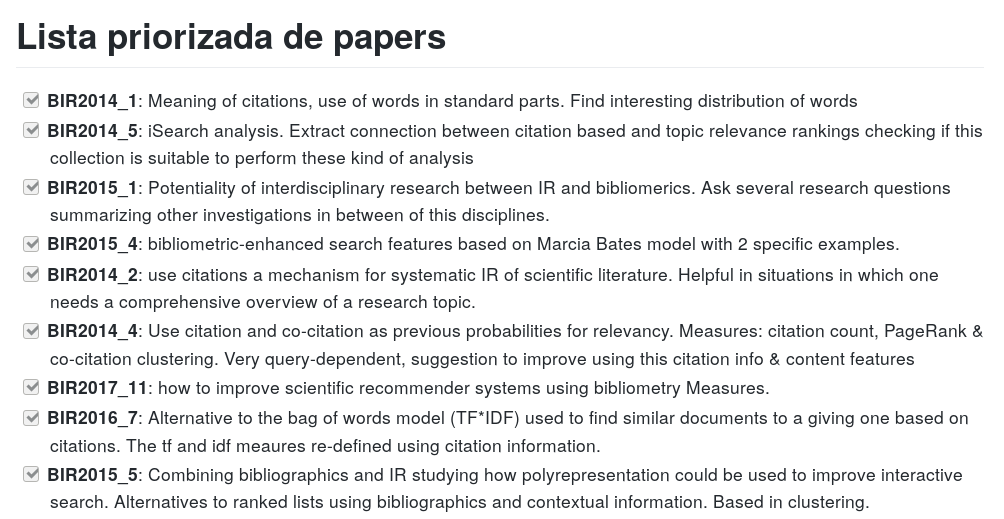
\includegraphics[width=\linewidth]{imagenes/lista_priorizada}
	\caption{Fragmento de la lista priorizada creada}
\end{figure}

\section{\textit{Sprint} 2}
Para el segundo \textit{sprint} plantee el indagar en la \acrshort{RI} e ir introduciendo la bibliometría. Sus objetivos concretos son: 

\begin{itemize}
	\item Leer los primeros 17 papers de los \acrshort{BIR} resumiendo y extrayendo ideas interesantes para el proyecto.
	\item Buscar información sobre medidas bibliométricas (Citas, índice h combinado...)
\end{itemize}

A partir de la lista priorizada fui leyendo los primeros artículos, el orden de esta lista lo fui alterando ya que con frecuencia al indagar en el trabajo este perdía o incrementaba su interés. Con el objetivo de poder aprovechar más estas lecturas fui creando una especie de resúmenes en los que anotaba los puntos más importantes que se trataban en el artículo, otros artículos relacionados de los que se hablaba o los resultados obtenidos con su trabajo. En la siguiente imagen se puede apreciar uno de estos "resúmenes":

\begin{figure}[h!]
	
	\centering
	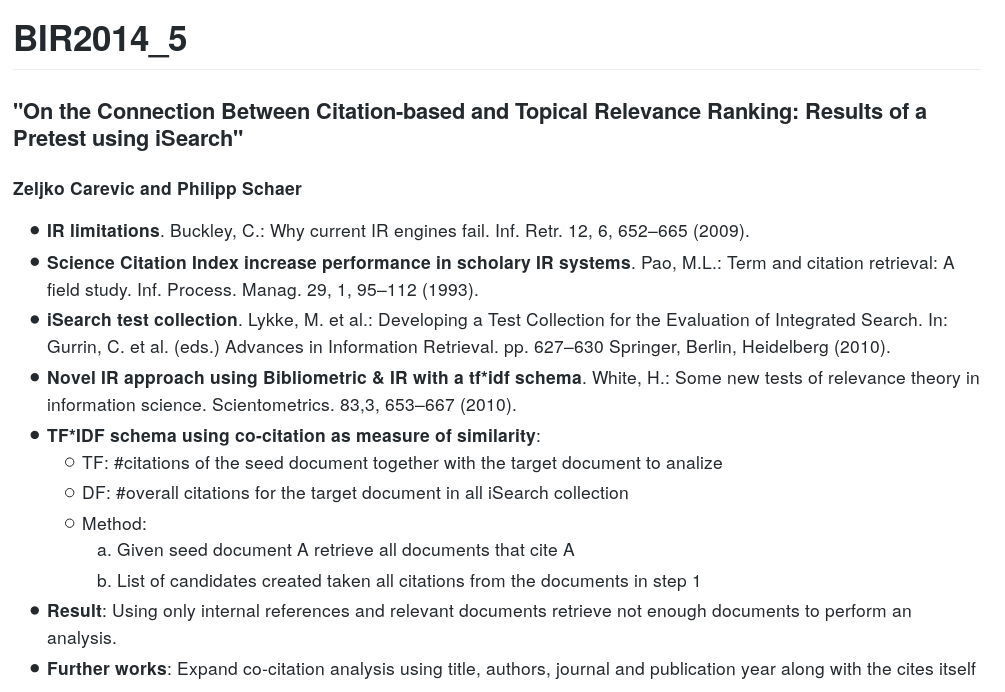
\includegraphics[width=\linewidth]{imagenes/paper_sumary}
	\caption{Ejemplo de resumen de uno de los papers}
\end{figure}

En este momento me empecé a introducir en el mundo de las medidas bibliométricas, ya que no tenía conocimiento previo alguno de que existiera esta disciplina siquiera, mediante la lectura de artículos iba descubriendo distintas medidas así como sus posibles aplicaciones a la \acrshort{RI} cuyo resultado final se encuentra sintetizado en la sección \nameref{sc:bibliometria} de la Introducción.

\section{\textit{Sprint} 3}
Ya en este punto decidí que estaba listo para ir documentando todo lo que había aprendido por ello en este \textit{sprint} me puse como objetivo escribir la introducción de este \acrshort{TFM}. Los objetivos concretos son:
\begin{itemize}
	\item Escribir la introducción del \acrshort{TFM}.
	\item Pensar un enfoque para el proyecto a desarrollar decidiendo que clase de sistema se desarrollaría.
	\item Continuar leyendo algunos artículos más de los \acrshort{BIR}.
\end{itemize}

Para asimilar y reflexionar sobre todo lo que había leído me puse a escribir la introducción de este trabajo ya que ello me ayudaría a pensar un enfoque correcto. También quería poder mostrar algo a mi tutor para obtener algo de \textit{feedback} por su parte.

Continué leyendo algunos trabajos más con lo que dí por concluida mi proceso de investigación. Uno de esos últimos trabajos fue \cite{DBLP:conf/ecir/SarolLS18} el cual me gustó especialmente ya que pasaban de un modelo teórico a algo más práctico, accediendo a la \acrshort{API} de Scopus e incluyendo ejemplos de su implementación en un repositorio de \textit{GitHub} lo que me llevo a plantear mi modelo híbrido combinando el sistema habitual de un sistema \acrshort{RI} con reordenamiento de resultados \textit{a priori} usando medidas bibliométricas y un ordenamiento \textit{a posteriori} utilizando un grafo de citación entre los documentos.

Desgraciadamente estos enfoques dependen ampliamente de la cobertura de medidas bibliométricas disponibles, por ejemplo me hubiera encantado poder probar una reordenación previa utilizando alguna \textit{altmetric} como el número de lecturas o descargas de un artículo, pero la plataforma que he utilizado para extraer los artículos no dispone de dichas medidas.

Como parte adicional de este sprint también estuve haciendo alguna pruebas con \glspl{framework} de búsqueda. Como he dicho previamente ya había utilizado \textit{Lucene} como parte de las prácticas de la asignatura \acrshort{GIW}, pero me pareció demasiado bajo nivel así que me centré en investigar otras alternativas. Encontré que las principales, que casualmente utilizaban por debajo \textit{Lucene}, eran \textit{\textbf{Solr}} y \textit{\textbf{\acrlong{ES}}}.

Buscando alguna comparativa \cite{ES_Solr} y comentarios de usuarios en plataformas tan reputadas como \textit{StackOverflow} \cite{ES_Solr_SO} parecía que se recomendaba \acrshort{ES} por ser más sencillo de usar por lo que realicé un breve tutorial \cite{ES_tutorial} que me gustó bastante ya que resulta realmente simple de usar y basta únicamente con realizar consultas sobre una \acrshort{API} \acrshort{REST} por lo que basta con hacer peticiones \acrshort{HTTP} con algún cliente simple como \texttt{curl}. Todo esto hizo que me decidiera por este servidor de búsqueda.


\section{\textit{Sprint} 4}

\section{\textit{Sprint} 5}

\section{\textit{Sprint} 6}

\section{\textit{Sprint} 7}

\section{\textit{Sprint} 8}